\documentclass{llncs}

\usepackage[utf8]{inputenc}
\usepackage{todonotes}
\usepackage{graphicx}
\usepackage{hyperref}
\usepackage{color}
\usepackage{amsfonts}
\usepackage{amsmath}

\usepackage{microtype}


\newcommand{\matodo}[1]{\todo[color=green!50]{#1}}
\newcommand{\cetodo}[1]{\todo[color=orange!50]{#1}}

\newcommand{\myparagraph}[1]{\noindent \textbf{#1}}

\begin{document}
\title{Running experiments with confidence and sanity}
%
%\titlerunning{Abbreviated paper title}
% If the paper title is too long for the running head, you can set
% an abbreviated paper title here
%
\author{
  Martin Aumüller\inst{1}%\orcidID{0000-0002-7212-6476} 
  \and
  Matteo Ceccarello\inst{2}%\orcidID{0000-0003-2783-0218}
  }
%
\authorrunning{M. Aumüller and M. Ceccarello}
% First names are abbreviated in the running head.
% If there are more than two authors, 'et al.' is used.
%
\institute{
  IT University of Copenhagen,
  Denmark\\
  \email{maau@itu.dk}
  \and
  Free University of Bozen, Italy\\
  \email{mceccarello@unibz.it}}
%
\maketitle              % typeset the header of the contribution
%
\begin{abstract}
Analyzing data from large experimental suites is a daily task for
anyone doing experimental algorithmics.
In this paper we report on several approaches we tried for this 
seemingly mundane task in a similarity search setting, reflecting on the many errors and consequent
mishaps.

We conclude by proposing a workflow, which can be implemented using several
tools, that allows to analyze experimental data with confidence.

\keywords{Experimental algorithmics; Experimental analysis%; data analysis
}
\end{abstract}

\section{Introduction}

One of the peculiar aspects of \emph{experimental algorithmics}~\cite{DBLP:journals/jucs/MoretS01}
is that the object of the study (an algorithm and its implementation)
is often crafted by the same people carrying out the analysis.
This has the advantage that the insights obtained from preliminary
investigations of early versions of an algorithm can be used to improve the
algorithm itself.
In fact,
the understanding required for an implementation may uncover features of the
algorithms that would otherwise go unnoticed~\cite{DBLP:journals/jucs/MoretS01}, giving
insights about aspects not easily described by theoretical
models of computation~\cite{DBLP:journals/cacm/McGeoch07}.
At the same time, this feedback-based process leads to the
accumulation of obsolete data, referring to old versions of
algorithms and their implementations.
Not mixing results from different versions of
an algorithm or implementation is an obvious requirement, which
however requires some care in practice.
In fact, a study often involves different algorithms and datasets,
each evolving at a different pace: weeks-old results might be up to date
for one algorithm, and obsolete for another.


As we shall see, the literature is mainly concerned with the design 
and analysis of
experiments
and with reproducibility.
In this paper, instead, we report on our experience with the day to day
tasks that have to be carried out in between those three tasks, and
the approaches we developed to tackle the perils and frustrations of this 
often menial work.

We don't advocate for any specific technology. Rather, we propose a workflow
that can be implemented with a variety of tools that can be easily integrated
into existing setups. We demonstrate such a setup with a toy project that concerns an efficient implementation of a brute-force nearest neighbor search.

\section{Related work}

Moret and Shapiro~\cite{DBLP:journals/jucs/MoretS01} advocate for the
importance of complementing the theoretical analysis of algorithms
with their implementation.
McGeoch~\cite{DBLP:reference/algo/McGeoch08} gives several guidelines on how to
design and carry out experimental analyses of algorithms.
The book~\cite{DBLP:books/sp/2010BCPP} collects several contributions
on the characterization and analysis of algorithm performance.
Earlier, a Dagstuhl seminar has been devoted to the discussion of the
experimental evaluation of algorithms~\cite{DBLP:conf/dagstuhl/2000ea}.
More recently, a structured approach to the design and evaluation
of experiments has been discussed in~\cite{DBLP:series/ncs/Bartz-BeielsteinP14}.
%
% Experimental studies can be influenced by contingent aspects
% of the evaluation:
% Bartz-Beielstein~\cite{DBLP:reference/sp/Bartz-Beielstein15} discusses
% the issue of generalizing the conclusions of experimental studies.
% %
% McGeoch and Moret~\cite{DBLP:journals/sigact/McGeochM99} and Sanders~\cite{DBLP:conf/dagstuhl/Sanders00}
% focus on the reporting of experimental results.

In recent years there has been a discussion about the lack of reproducibility
of research findings in several areas, including 
computer science~\cite{DBLP:journals/cacm/CollbergP16,Hutson725}.
Much effort has been devoted to finding a solution to this issue. Several
contributions have been collected in~\cite{stodden2014implementing} 
and~\cite{kitzes2017practice}.
Among the tools to support reproducible research, 
VisTrails~\cite{DBLP:conf/sigmod/CallahanFSSSV06} allows to
explicitly define reproducible workflows.
\texttt{knitr} and \texttt{Jupyter} take a \emph{literate programming}
approach, allowing experiment's code, analysis, and text to be interleaved
in a single "executable" document.
To solve the issues deriving from software dependencies,
some tools aim at capturing the execution
environment at runtime~\cite{DBLP:journals/cse/Guo12,davison2014sumatra,DBLP:journals/jossw/RampinCSFS16},
while others such as Docker~\cite{DBLP:journals/sigops/Boettiger15}
and Singularity~\cite{kurtzer2017singularity} follow a \emph{declarative}
approach, where the description of the execution environment is part
of the code base


\section{Challenges in running large scale experimental evaluation}
\begin{figure}[t]
  \centering
  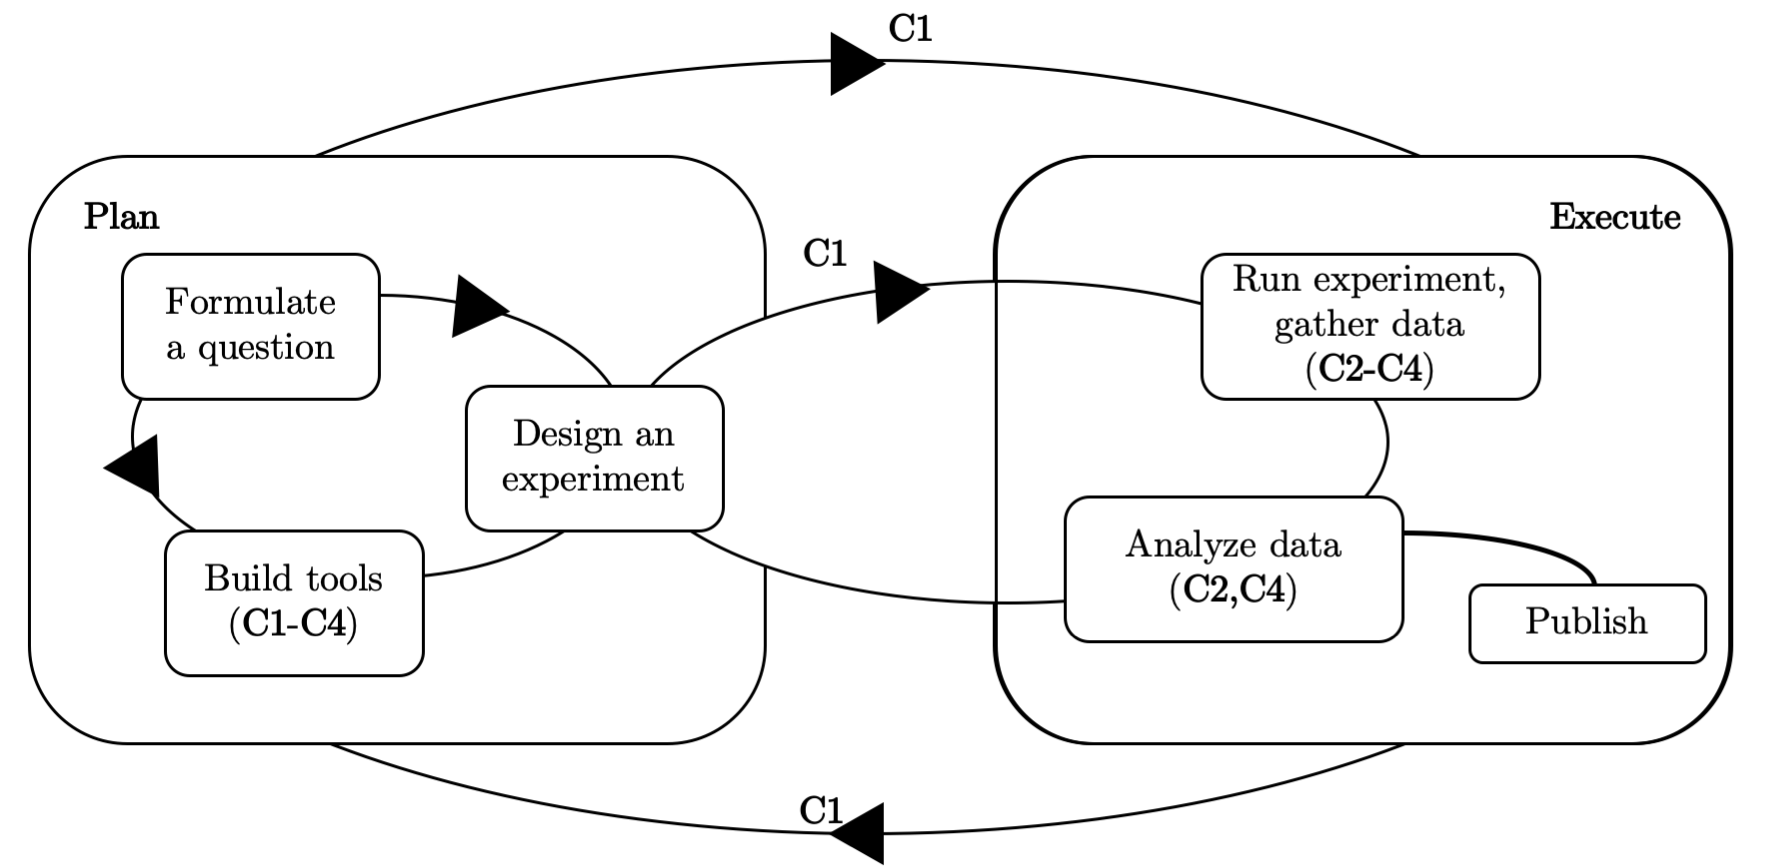
\includegraphics[width=0.8\textwidth]{figs/experiment_scheme.png}
  \caption{Overview of the different stages of an experimental study; adapted from~\cite{DBLP:reference/algo/McGeoch08} by adding challenges to individual tasks and feedback loops.}
  \label{fig:overview}
\end{figure}
We define the following challenges in the  evaluation of large-scale experiments:
\begin{enumerate}
  \item[(C1)] \textbf{Feedback Loops-by-Design.} Implementations and tools support the iterative nature of an experimental study.
  \item[(C2)] \textbf{Economic Execution.} Exactly those experiments that change through code changes have to be re-run, but nothing else. 
  Moreover, only the changing parts of the experimental evaluation should be recomputed.
  \item[(C3)] \textbf{Versioning.} The ability to go back in time and compare old results to more recent ones, finding regressions or bugs; the workflow is \emph{append-only}.
  \item[(C4)] \textbf{Machine Independence.} Code and tools are designed in a way that allow them to run in a general setting.
  \item[(C5)] \textbf{Reproducibility-by-Design.} We strive for an automatic workflow that processes an experimental setup into measurements used for evaluating the experiment. Results to be included into a publication should not require manual work to transform these measurements into tables and plots.
\end{enumerate}
%
%We will detail these challenges in the following. 
%
Typically, an experimental evaluation spans several weeks, if not months. An overview of a typical experimental evaluation is given in Figure~\ref{fig:overview}. 
During this time, the experiments being run have different meanings: early
on during initial development, experiments are useful to find out the most
appropriate parameter ranges, find bugs, and check assumptions; later on,
experiments collect the results of the study.
This is not a process that proceeds linearly from start to finish. 
Rather, the analysis of the results might prompt the modification of an algorithm
or dataset, or the introduction of new algorithms and datasets into the study,
followed by a new round of experiments.
Together with the algorithms and the datasets, also the parameterizations and the
quantities being measured are subject to evolution during the lifetime of a project (C1).

For the analysis to be sound, it is of paramount importance not to 
mix results related to different versions
of the algorithms and datasets (C3), in particular when experiments are run on a set of different machines (C4). 
The simplest solution would be to re-run the entire experimental suite whenever
something is modified. 
This usually takes a very long time, and a change might affect 
only a small part of the results, making this solution wasteful of time, energy, computational resources and money if computing resources are rented (C2). 
A potential solution might be to divide the experimental suite in smaller
components, each investigating a particular aspect, re-running only those 
affected by a change.
While this works in the short term, as the experimental study progresses
the subdivision of the experimental suite will evolve with it, leading to the
need of re-arranging the results.
On the other hand, manually re-running only parts of an experimental suite,
while reusing results from old runs, requires much care in order to exclude
obsolete results from the analysis, undermining the confidence in the soundness
of the whole analysis.
The situation worsens in the rushed final days preceding a submission:
some last minute changes are made, there is no time to re-run all the experiments,
the possibility of erroneously mixing results is very concrete. Additionally, reviewers will often demand running a new set of experiments, reporting on some other quality measures, or experimentation using different computer architectures (C2, C3, C4). \emph{Reproducibility-By-Design} (C5) requires that such wishes can be accommodated since the whole process from starting at an experimental design to a published table or figure is automated.

As for the analysis itself, it is usually executed on a machine different from the
experimental code, using a different programming language (C4).
The input of the analysis is the set of results produced by the experimental suite,
which is usually quite large due to the fact that many parameter combinations
need to be evaluated.
While the analysis code may not need the computational resources of the 
experimental code, it still needs to execute reasonably fast, in order to be able
to examine the results interactively.
This implies that the results produced by the experiments need to be 
stored in a convenient
format that is at the same time easily manageable, convenient to transfer, and efficient to access (C2, C4).



\section{Case study: Engineering a Linear Scan}

As our toy project, we engineer a nearest neighbor search algorithm that just carries out a linear scan over the dataset. 
Formally, we are given a dataset $S \subset \mathbb{R}^d$ of $n$ points in a $d$-dimensional space with a distance measure $\text{dist}\colon \mathbb{R}^d \times \mathbb{R}^d \rightarrow \mathbb{R}$, such that given a query $q \in \mathbb{R}^d$ we want to return a point $p \in S$ that minimizes dist$(p', q)$ over all $p' \in S$.
Solving this problem via a linear scan is a straight-forward exercise in an introduction to programming class: Compare all points $p' \in S$ one by one to $q$, and keep track of the point that is closest to $q$. This results in a running time $O(nd)$ for a single query.

To make this problem more interesting, we consider engineering choices to speed up a linear scan under inner product similarity $\text{dist}_{\text{IP}}(p,q) = \sum_{1 \leq i \leq d} x_i y_i$ on unit vectors, similar to Cosine similarity.
For the purpose of this project, we consider (i) input representation, (ii) parallelization, and (iii) saving distance computations as factors of the experiment.

\myparagraph{Input representation.}
A vector in $\mathbb{R}^d$ is traditionally represented as $d$ 64-bit floating point values (\texttt{double}) or 32-bit floating point (\texttt{float}). Since we guarantee $0 \leq x_i \leq 1$ for normalized vectors, we also consider a 16-bit representations of the value $\lceil x_i \cdot 2^{16} \rceil / 2^{16}$ (which could of course affect the accuracy of the result.)

\myparagraph{Parallelization.}
Naïvely, the CPU has to carry out $d$ multiplications and $d-1$ additions to compute the distance of two vectors.
However, we notice that the structure is inherently parallel because the multiplications are data independent. This is an ideal setup for using so-called SIMD instructions (single instruction multiple data). 
We split up each vector into blocks of size $B$, and carry out $d/B$ parallel multiplications, $d/B$ parallel additions to aggregate terms in a register of size $B$, and one horizontal sum. 
Depending on the CPU architecture used in the experiment, $B$ is usually 128, 256, or---very recently---512 bits.

\myparagraph{Saving Distance Computations.} Computing the distance 
between two vectors is certainly the most expensive operation in our linear scan. 
Hence, if we could decide for a data point $p'$ that it probably is not the nearest neighbor faster than carrying out a distance computation could increase the performance of our linear scan. 
We include experiments with a 64-bit sketch using SimHash with probabilistic quality guarantees in our experiments (see Appendix~\ref{app:sketches}).

\medskip

We consider this toy project representable for an experimentation task in a similarity search setting. 
The different choices of input representation, parallelization, and distance filter methods provide an evolutionary setting in which we start with a standard linear scan and add features to the code base one by one. 
From starting with a measurement of running time, we quickly end up focusing on the quality of the achieved result when using a low-precision input representation, or analyzing the effectivity of the sketch by counting distance computations.
The experiment has to be carried out on different machines because of the hardware dependencies, which might mean to rent cloud instances to carry out measurements on recent hardware with $B = 512$ bit AVX512 support. 

Our code is provided at \url{TODO}. For the scope of this paper, we consider the \emph{support code} that takes care of handling the setup as the main contribution. The evaluation of the this toy project is give in~\ref{app:linear:scan}.

\section{Approaches to experimental evaluation}
We now describe a workflow we developed to address the challenges outlined
in the previous sections, demonstrating it with our case study.
We split up the discussion into different dimensions of running 
a successful experimental study. 
These dimensions are summarized in Figure~\ref{fig:discussion}. 
In the following, each dimension will be introduced with general
guidelines and a discussion of our actual solution. 

\begin{figure}[t!]
  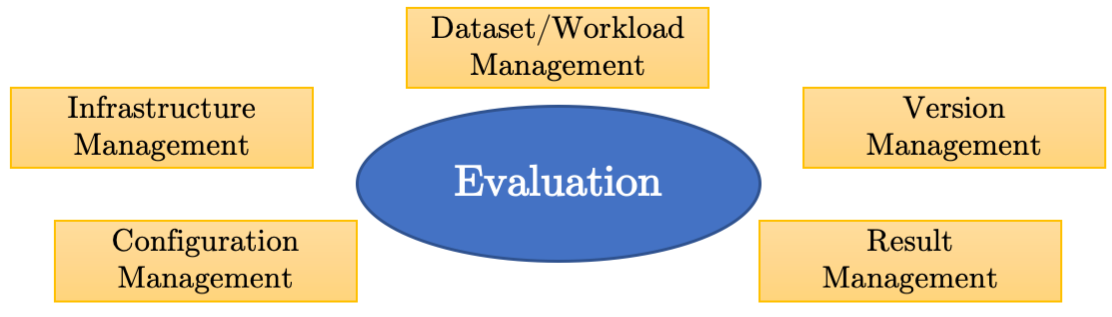
\includegraphics[width=\textwidth]{figs/discussion_points.png}
  \caption{Dimensions for running large-scale experimental evaluations.}
  \label{fig:discussion}
\end{figure}

\subsection{Manage the datasets and workloads efficiently}

\begin{itemize}
\item Dataset download and preprocessing should be automated as much as possible,
  ideally with a single script responsible to manage all the datasets.
  This makes reproducibility easier, allows to share preprocessing steps between similar datasets,
  makes it easy to relocate the experiments on a different machine, and makes all the
  decisions about datasets explicit.
  Furthermore, it enables the community to change the datasets to observe how these changes
  are reflected in the experiments.
\item It must be possible to create all datasets locally, 
  but the preprocessed datasets should also be shared, for instance using plain 
  \texttt{http} or a service such as \texttt{S3}.
  This makes it easier for collaborators, reviewers, and the community to re-run the
  experiments without incurring the set-up cost of the datasets.
\item Datasets should be annotated with meta-data necessary in the evaluation, 
  such as workloads and the related ground truth answers.
\item To ease debugging, a small dataset of random data that can be created in a few
  seconds should also be included. This dataset can be run via Continuous Integration (CI), and results on it can be stored to enable regression testing. 
\end{itemize}
%
In our code, the main C++ code calls a Python script ({\tt datasets.py}) that takes care of preprocessing datasets in a well-defined manner. It checks for the existence of a shared dataset (of the same version) and computes it locally if such a dataset is not available. It supports that creation of tiny random datasets that allows to run all parts of the workflow on actual data. The query set that is latter used for experimentation is created in this process as well, and data is stored as an {\tt HDF5} file for efficient processing in many different programming languages.

\subsection{Manage the experimental configurations clearly}

\begin{itemize}
\item Never run experiments from the command line. Direct command line execution
  should be limited to testing.
\item Experiments should be described in one or more files. This makes it easier
  to reproduce the entire experimental suite. There are several options, which we both 
  demonstrate in the associated code:
  \begin{itemize}
    \item Files in a declarative language such as YAML listing all the combinations of
    parameters to be tested. These files are then interpreted by a script that spawns
    the appropriately configured experimental code. This approach has the advantage of
    being declarative, and the disadvantage of requiring some additional software.
    \item Shell scripts that directly invoke the experimental code using 
      the appropriate parameters. This is a more procedural approach, which however has
      the advantage of requiring very little setup.
  \end{itemize}
\item All the aforementioned experimental files should be tracked with version 
  control along with the code. Before running the experiments, any pending changes should be committed.
\item There should be a mechanism allowing to skip already-run configurations.
  This allows both to save time (C2) without having to continuously edit
  the configuration files to remove the configurations that do not need to be run.
\end{itemize}
%
We provide the example files that we used in Appendix~\ref{app:experiment-file}. While a direct experimental file written in Bash is straight-forward, the YAML structure gives a much more structured overview. The YAML file is run through an additional Python script that invokes the main implementation with the correct parameters. Using versioning and the result database (Subsection~\ref{sec:manage-experiments}) the code can decide whether an algorithm has to be rerun.

\subsection{Infrastructure management}

Any implementation will likely depend on many different environmental settings, such as the correct versions of libraries/compiler/OS.
To allow a machine independent workflow, we suggest to:
\begin{itemize}
  \item Provide a containerized development environment\footnote{Recently, such environments are included in programming IDE such as \url{https://code.visualstudio.com/docs/remote/containers}}.
  \item Consider different container formats for running experiments~\cite{arango2017performance}.
  \item Use continuous integration to test all parts of the workflow.
\end{itemize}
%
Our code provides a {\tt Dockerfile} that installs a well-defined Linux environment and sets up the correct compilers and libraries. 
Each component is run from the local system via a {\tt dockerrun} script that will run the intended process within the container. 
The main program has a simple interface:\cetodo{This text now is unrelated to the above, since we removed the section about the code infrastructure. Shall we remove it?} it implements the linear scan, the logic for reading the dataset, and the logic to communicate with the database. 
It will run the pre-defined workload and report the running time and the indices of the nearest neighbor for each query.

\subsection{Version everything}

To address challenges (C2) and (C3), version control systems might not be sufficient,
since source code revisions lack both a semantic meaning and a total order.
Furthermore, different components of a project might 
evolve independently, thus
needing independent versioning to address challenge (C2).
Therefore, we suggest to keep track of the versions of individual components of the project,
including datasets, algorithms, and database schemas, alongside the versioning provided
by the version control system.

In our code, each dataset and database schema provides their own version number. Additionally, components of the implementation such as input representation type or SIMD definitions are versioned. This allows us to map each parameter set for the linear scan to a unique identifier. As an example, during continuous integration we found a bug that only affected the AVX2 inner product computation with floating point numbers. An update of the version number of this part of the code led to a re-run of all parameter configurations that used that particular combination. Each measurement obtained is versioned with its \emph{git identifier}, the algorithm version in question, and the dataset version. 
\matodo{Downside: Manual work that might be error-prone.}
\cetodo{A better approach might be to make every component a class (with
distance functions turned into functors) and make every one of them implement 
a `Version` template. I tried it but I find templates in C++ very unnerving :-) }

\subsection{Manage the experimental results thoughtfully}
\label{sec:manage-experiments}

As for the management of experimental results, structured text file formats like CSV address challenge (C4), but are expensive to parse and require to be fully loaded in main memory prior to the analysis, even when only a subset is needed.
Moreover, it is hard to evolve the structure of these files together with 
the project.

\begin{itemize}
\item Use a database to store the results: it presents data 
conveniently indexed and removes the need for expensive parsing. 
\item Use schema migrations the database can evolve along with
the rest of the project (C3), as demonstrated in our case study's code.
\item For simple projects, an embeddable database like SQLite\footnote{\url{https://sqlite.org}}
addresses challenge (C4): the results are stored in a single file which can be easily moved
between machines, and many languages used for the analysis (like Python and R) provide
facilities to access it, as shown in our code. 
For larger projects, where experimental code is executed on different machines, a database with
a client-server architecture\footnote{Such as PostgreSQL: \url{https://www.postgresql.org}} 
might be more suitable.
\item The experimental code can query the database to detect whether an experiment has already been run with the current version (C2).
\item Track the \emph{provenance}~\cite{BunemanKW01} of each result, by storing alongside the parameters also the configuration file (and its version) that generated the result (C5).
\item
By means of database views we can enforce that the analysis code
has access only to the most recent results related to each algorithm/dataset (C3): our code
demonstrates how to embed a query in the database so to present only the results related to 
the most recent version of algorithms and datasets.
\end{itemize}

\section{Conclusions}

\paragraph*{Acknowledgements.} Many of the ideas of our toy project were originally developed by Michael Vesterli for PUFFINN~\cite{puffinn}.

\bibliographystyle{splncs04}
\bibliography{references}

\appendix

\section{Experimental Example: Bash vs. YAML}
\label{app:experiment-file}

\section{Review: Linear scan using 1-bit sketches via SimHash}
\label{app:sketches}

Charikar described in~\cite{Charikar02} the well-known \emph{SimHash} scheme that maps a unit vector $x \in \mathbb{R}^d$ to $\{0,1\}$. 
It works by choosing a random $d$-dimensional normal vector $a \sim \mathcal{N}(0, 1)^d$   and mapping $x$ to the indicator variable $[ax \geq 0]$. For two unit vectors $x,y$, the probability of mapping to the same bit is $1 - \text{arccos}(xy)/\pi$.

Assume we choose 64 independent SimHash functions to produce a 64-bit sketch. The number of differences between two vectors $x$ and $y$ is distributed as $\text{Bin}(64,\text{arccos}(xy)/\pi )$ and it is easy to derive thresholds $\tau$ for a failure probability $\delta > 0$ such that with probability at least $1-\delta$, the number of difference between $x$ and $y$ is at most $\tau$. (In the simplest case, we can just use standard Chernoff bounds that one such choice for $\tau$ is $64\text{arccos}(xy)/\pi  + \sqrt{192 \ln (1/\delta)\text{arccos}(xy)/\pi}$.)

To find a nearest neighbor of a given point $q$ with probability at least $1-\delta$, we carry out a linear scan by first checking the 64-bit sketch of the current data point $p$ and the query point, and only if we cannot rule out that $p$ could be the nearest neighbor of $q$, we carry out the actual distance computation. The threshold $\tau$ is set based on the inner product of the current closest nearest point and the query point as above.


\section{Evaluation of our Engineered Linear Scan}
\label{app:linear:scan}

\myparagraph{Experimental setup.}

\myparagraph{Evaluation.}

Figure~\ref{plot:eval}(top) shows differences between a brute-force linear scan based on the input representation and the vectorization technique. 

Figure~\ref{plot:eval}(middle) shows how throughput adapts to the recall level. 

Figure~\ref{plot:eval}(bottom) relates filters using no and avx2 vectorization.

\begin{figure}
  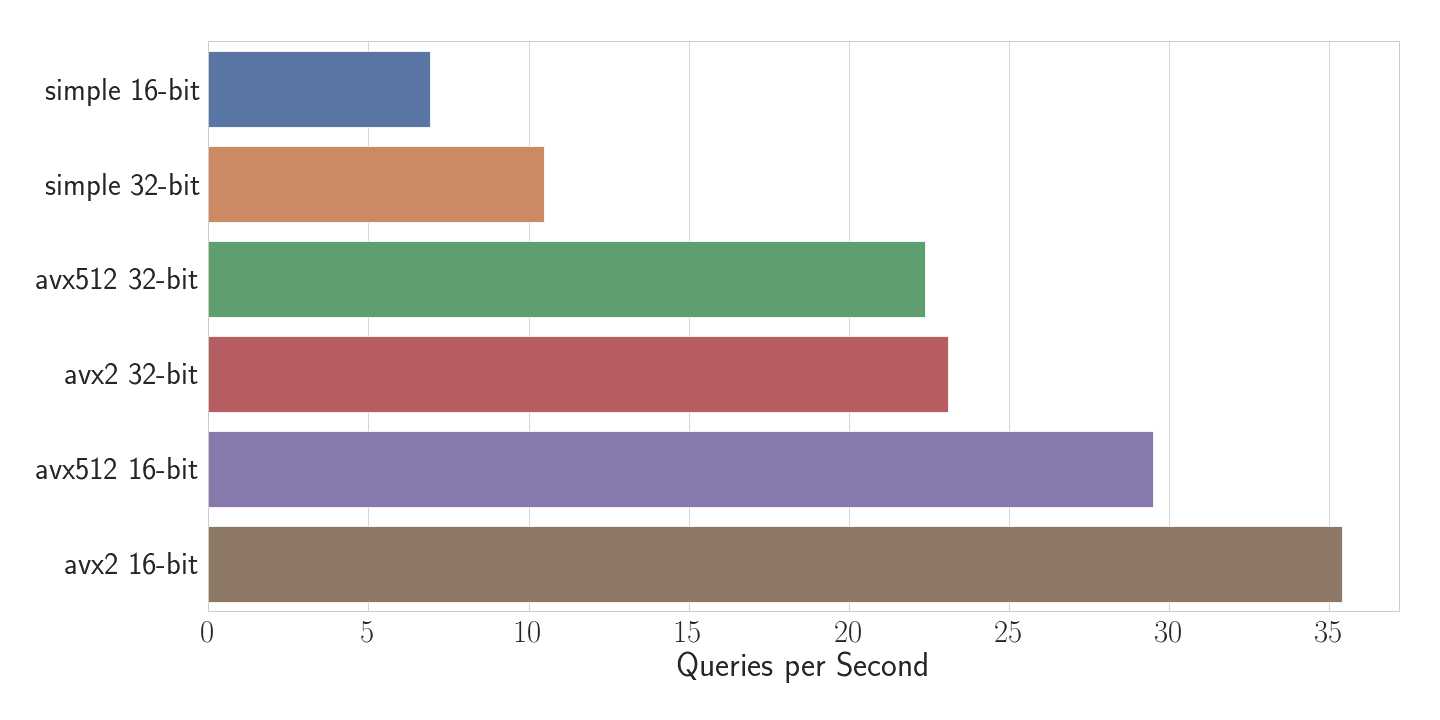
\includegraphics[width=\textwidth]{figs/linearscan_no_filter.png}
  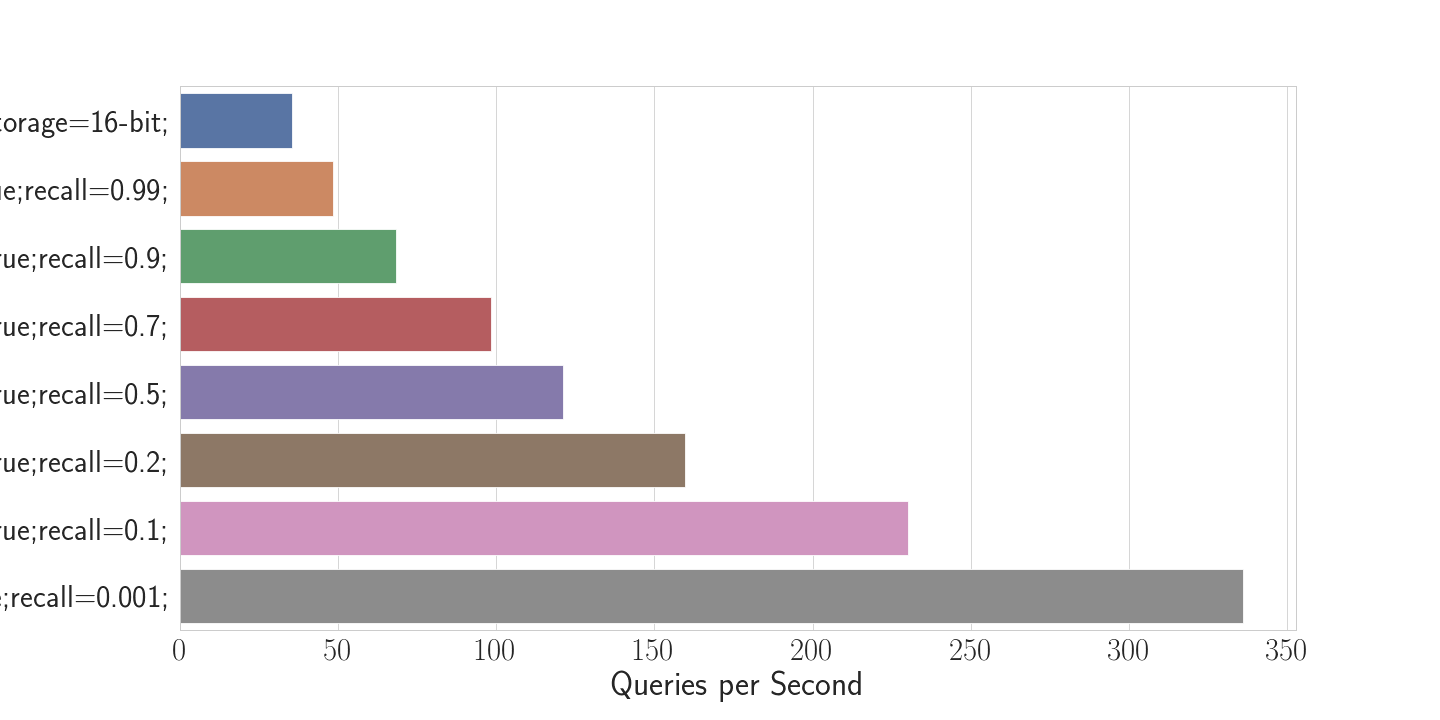
\includegraphics[width=\textwidth]{figs/16bit_filter.png}
  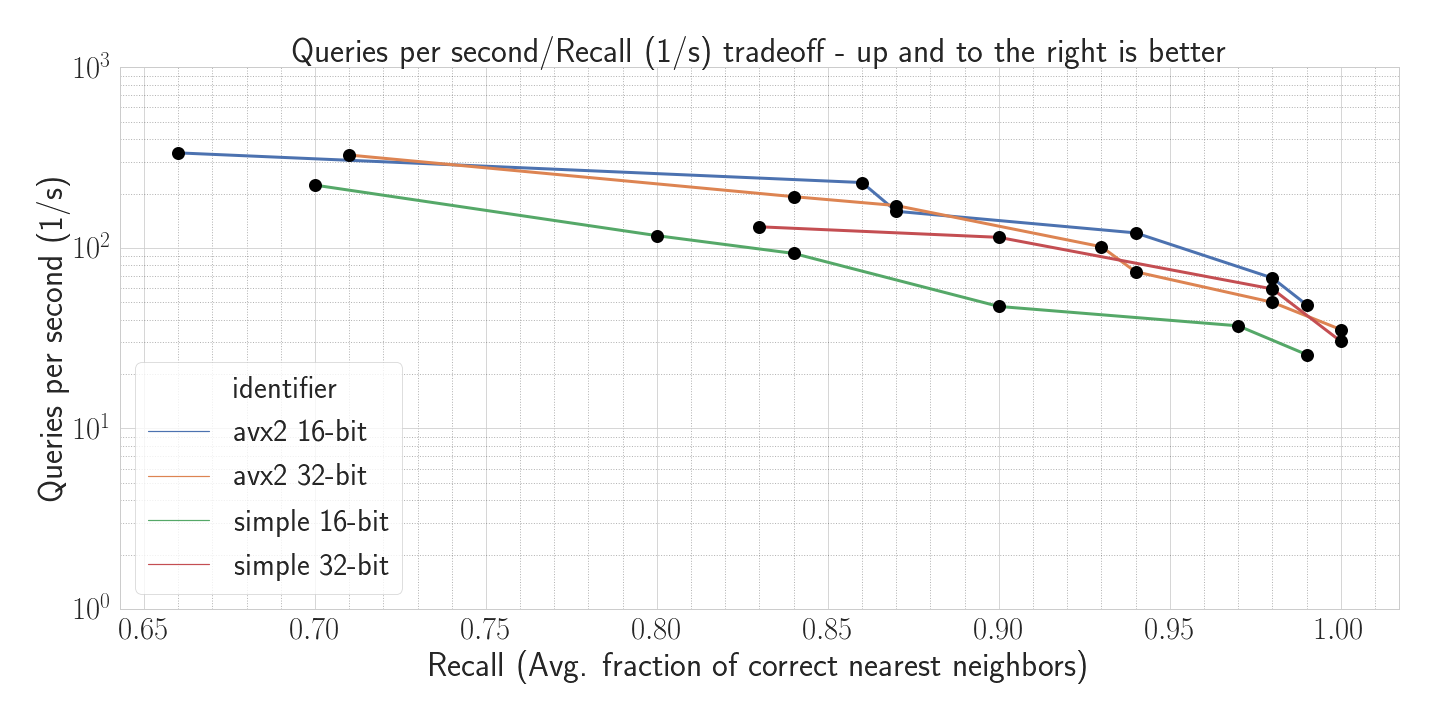
\includegraphics[width=\textwidth]{figs/avx2_16vs32bit.png}
  \caption{Overview of our experimental results.}
  \label{plot:eval}
\end{figure}


\end{document}

